\section{Analysing data}
\label{sec-analyse}

The \textsf{Geant-val} website provides two ways of viewing and comparing results:

\begin{figure}[h]
    \centering
    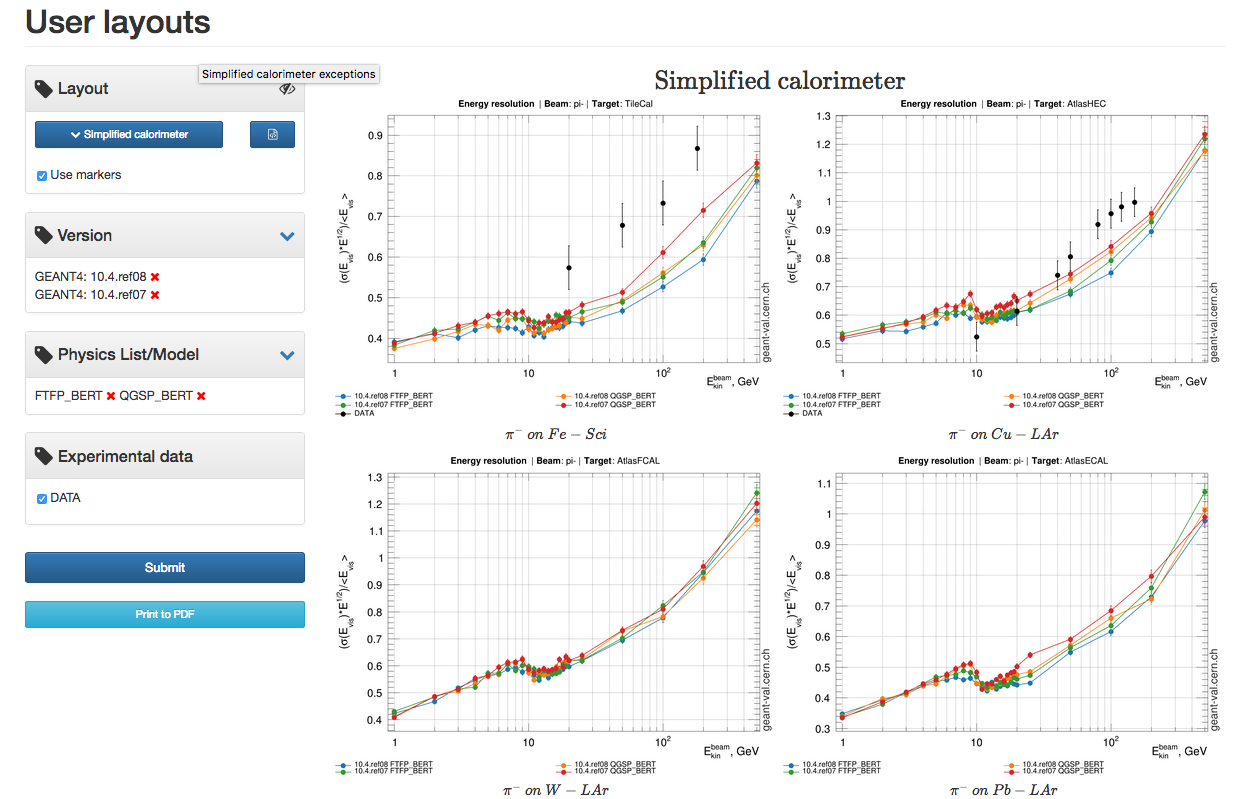
\includegraphics[width=0.8\textwidth,clip]{layout_sc.png}
    \caption{Example of user defined layout for the Geant4 "simplified calorimeter" test showing test results for two Geant4 reference releases - 10.4.ref07 and 10.4.ref08.}
    \label{fig:layouts}
\end{figure}

\textit{Statistical comparisons} page (see Fig.~\ref{fig:statcomparison}) allows one to perform comparison of simulation with compatible experimental results using statistical tests. % It displays results of statistical comparison for pairs of plots with the same parameters' values.
Currently $\chi^2$ ($\chi^2/n.d.f.$, $\chi^2$ probability) and Kolmogorov-Smirnov (KS Max(D), KS probability) tests are implemented. All computations are performed asynchronously on the client side using JavaScript WebWorkers. For this purpose, JavaScript code to perform $\chi^2$ and Kolmogorov-Smirnov tests have been written, and their results cross-checked against the same statistical techniques implemented in the ROOT framework.

\begin{figure}[h]
    \centering
    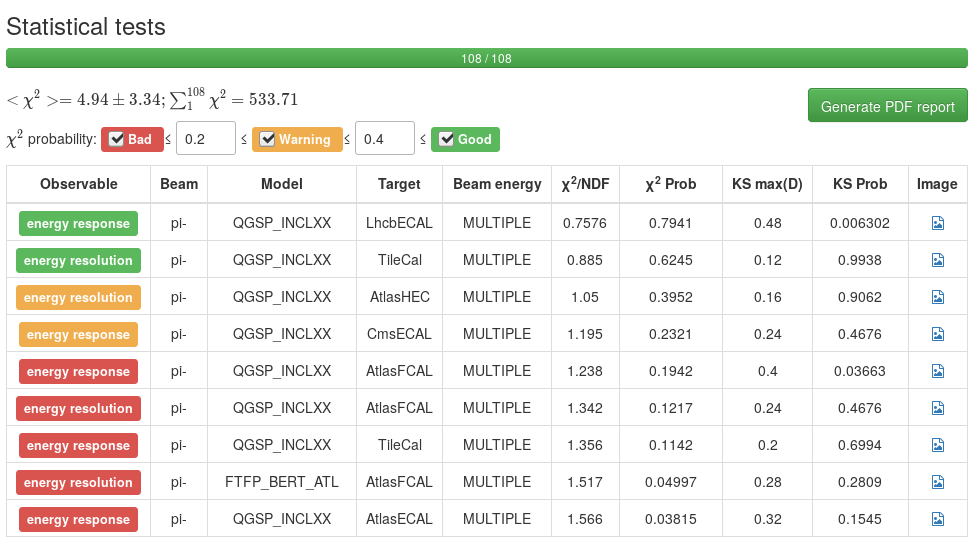
\includegraphics[width=0.8\textwidth,clip]{statcomparison.png}
    \caption{Example of statistical comparison between two official Geant4 releases, 10.5.beta01 and 10.4.p02, for the "simplified calorimeter" test.}
    \label{fig:statcomparison}
\end{figure}

\textit{User layouts} page (see Fig.~\ref{fig:layouts}). Some Geant4 tests produce hundreds of different plots, but for fast "visual" validation it is often enough to compare only a small well-defined subset of them. The \textit{User layout} is an XML file describing what plots should be displayed and how should they be laid out on a page. User can use one of the existing layouts or define their own one (see Appendix~\ref{adx:XML-format}).
